%%%%%%%%%%%%%%%%%%%%%%%%%%%%%%%%%%%%%%%%%%%%%%%%%%%%%%%%%%%%%%%%%%%%%%%%%%%%%%%
%
% Harvard ALM Thesis
%
% Author: Tony Allen (cyril0allen@gmail.com)
%
%%%%%%%%%%%%%%%%%%%%%%%%%%%%%%%%%%%%%%%%%%%%%%%%%%%%%%%%%%%%%%%%%%%%%%%%%%%%%%%

\documentclass[12pt]{article}
\usepackage[pdftex]{graphicx}
\usepackage{setspace,caption}
\doublespacing


% Default margins are too wide all the way around. I reset them here
\setlength{\topmargin}{1in}
\setlength{\textheight}{7in}
\doublespacing

\begin{document}
\author{Cyril Allen\\
Harvard Extension School}
\renewcommand{\today}{who knows}

%%%%%%%%%%%%%%%%%%%%%%%%%%%%%%%%%%%%%%%%%%%%%%%%%%%%%%%%%%%%%%%%%%%%%%%%%%%%%%%
\listoffigures

%%%%%%%%%%%%%%%%%%%%%%%%%%%%%%%%%%%%%%%%%%%%%%%%%%%%%%%%%%%%%%%%%%%%%%%%%%%%%%%
\section{Abstract}

% TODO

%%%%%%%%%%%%%%%%%%%%%%%%%%%%%%%%%%%%%%%%%%%%%%%%%%%%%%%%%%%%%%%%%%%%%%%%%%%%%%%
\section{Introduction}

With the advent of cloud computing, datacenters are making use of distributed
applications more than ever. Companies like Google use software such as
MapReduce to generate over 20 petabytes of data per day using very large
numbers of commodity servers [3]. Many other companies use large scale clusters
to perform various computational tasks via the the open-source MapReduce
implementation, Hadoop [4], or they can possess a virtualized datacenter
allowing them to migrate virtual machines between various machines for
high-availability reasons. As economics change for hardware, it is likely that
a scalable cloud will have the requirement to mix node types, which will lead
to higher performance/capacity nodes being mixed with lower
performance/capacity HDD nodes. This thesis presents an adaptive data placement
method in the Nutanix distributed file system (ADSF) which will attempt to
remedy the common problems found in many heterogeneous clustered file systems.

  \subsection{Motivation}

  A number of scenarios arise in heterogeneous Nutanix clusters that can
  degrade performance for an entire cluster. The currently replica disk
  selection logic in Stargate uses does not take into account a number of
  variables such as disparities in tier size, CPU power, workloads, and disk
  health among other things.

  Considering that a write is not complete until all replicas are written, the
  write's performance is at the mercy of the slowest disk and node.  There are
  several scenarios, both pathological and daily occurences, where a more
  robust replica placement heuristic is required. For the work in this thesis,
  I will focus on two orthogonal cases described below.

    \subsubsection{Interfering Workloads}

    An example of interfering workloads can take the form of a 3-node
    homogeneous cluster with only 2 nodes hosting active workloads as shown in
    Figure \ref{fig:workload_disparity}. In the current random selection scheme
    in use by the ADSF, writes are equally likely to place their replica on the
    other node with an active workload as they would be to place it on the idle
    node. This can impact performance on both the local and remote workloads as
    secondary writes will be slower on nodes whose resources are being utilized
    by their primary workloads. An adaptive replica placement scheme is needed
    to avoid the busy node and bias secondary replica placement on an idle
    node. 

    \begin{figure}[h!]
      \centering
      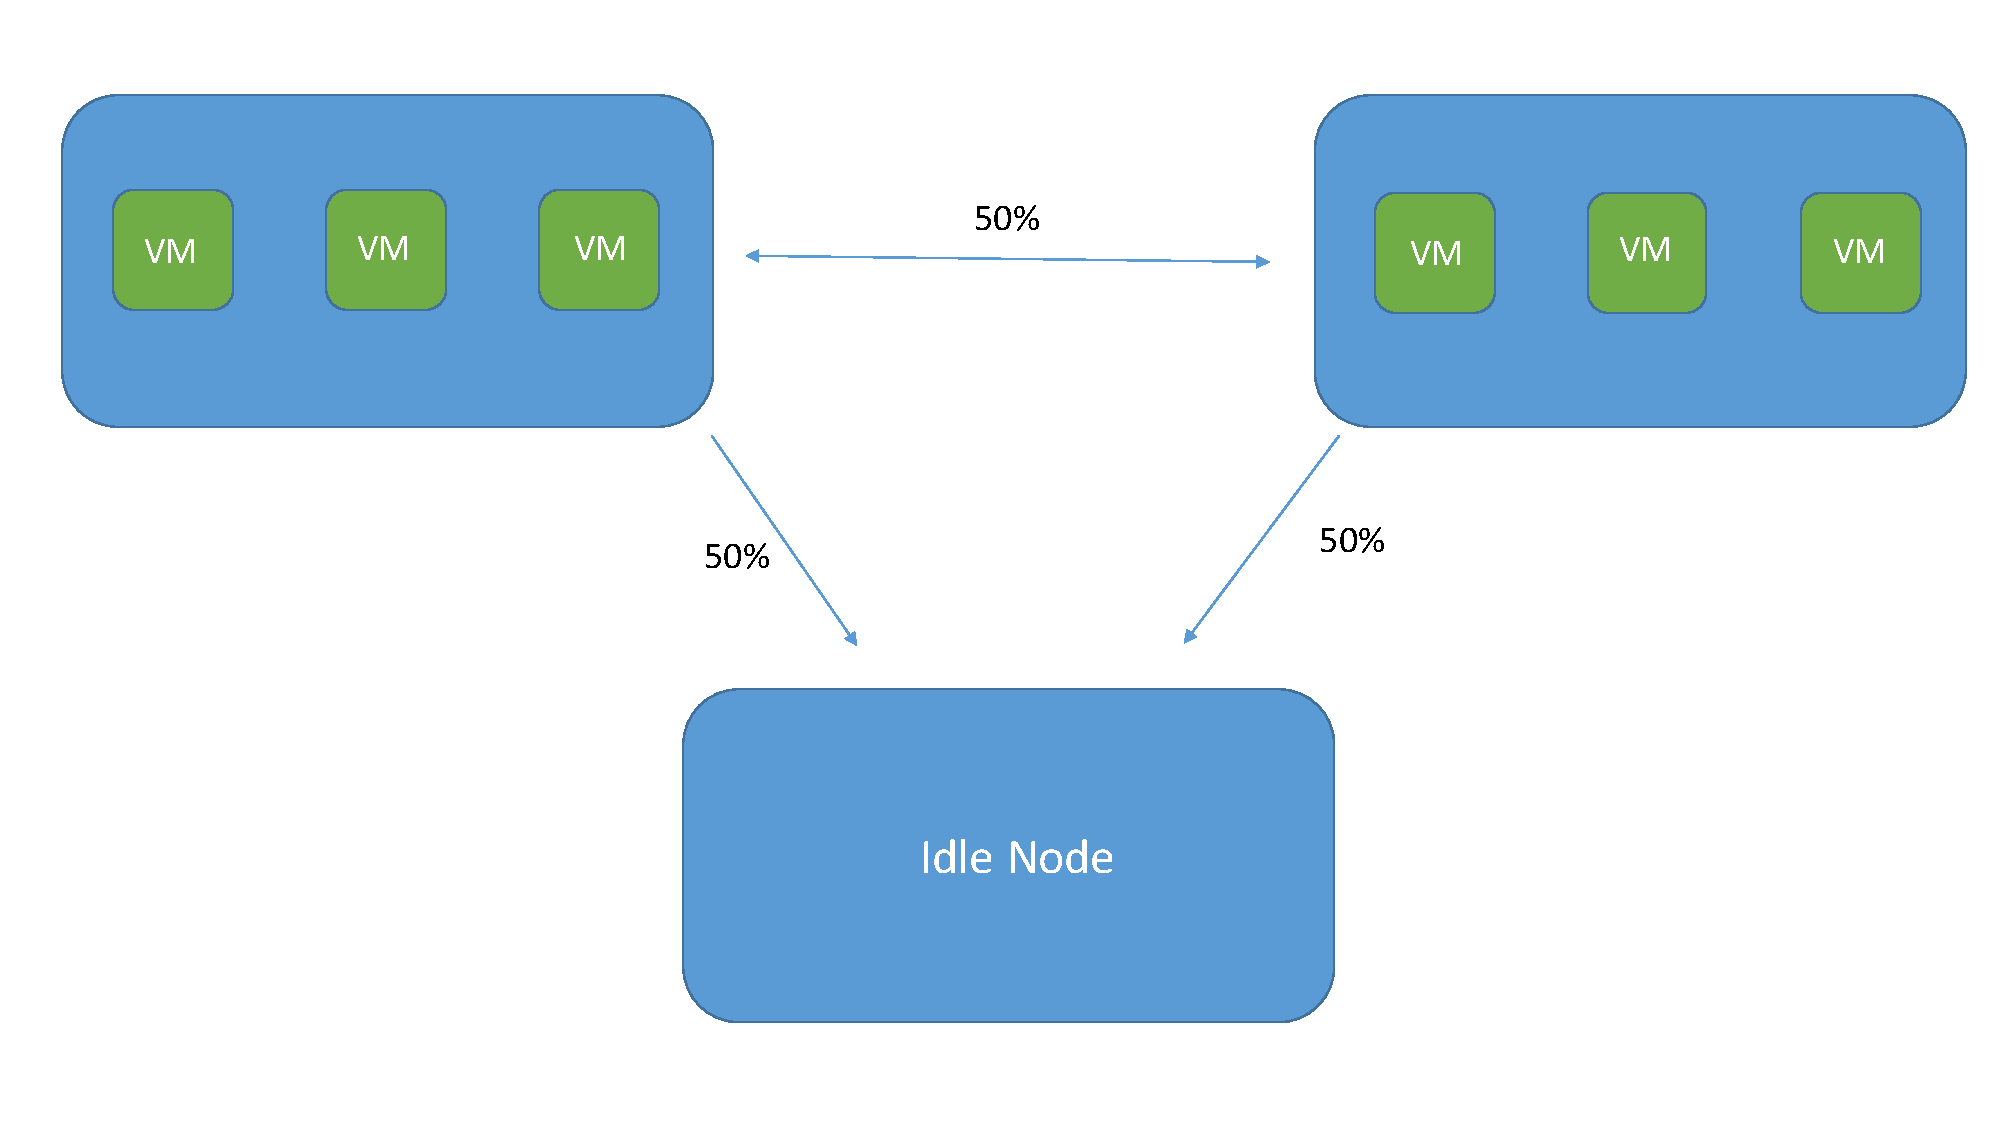
\includegraphics[scale=0.5]{images/homogeneous_workload_disparity.pdf} 
      \caption{A cluster with identical nodes running a heterogeneous workload.}
      \label{fig:workload_disparity}
    \end{figure}

    \subsubsection{Nodes with Tier Size Disparities}

    A cluster containing nodes with a tier size disparity are susceptible to a
    skew in node fullness, even if the workload on each node is identical. This
    can be illustrated via Figure \ref{fig:tier_size_disparity} where we have a
    3-node heterogeneous cluster with 2 high-end nodes and a single weak node.
    Suppose these high-end nodes have 500GB of SSD tier and 6TB of HDD tier and
    the single weak node has only 128GB of SSD tier and 1TB of HDD tier. If 3
    simultaneous workloads were to generate data such that the working sets of
    the workloads are 50\% of the local SSD tier, the weaker node is at a
    significant disadvantage. Given the current NDFS replica selection
    algorithm, we can expect 500GB of replica traffic to flood the weak node
    and fill up its SSD tier well before the workload is finished. This results
    in an inability for the workload on the smaller node to place its primary
    replicas locally and forces the workload to rely on remote CVMs, increasing
    latency. An adaptive replica placement heuristic would mitigate this issue
    by taking disk usages into consideration during the placement of secondary
    replicas and biasing placement of secondary replicas on the nodes with more
    free capacity.

    \begin{figure}[h!]
      \centering
      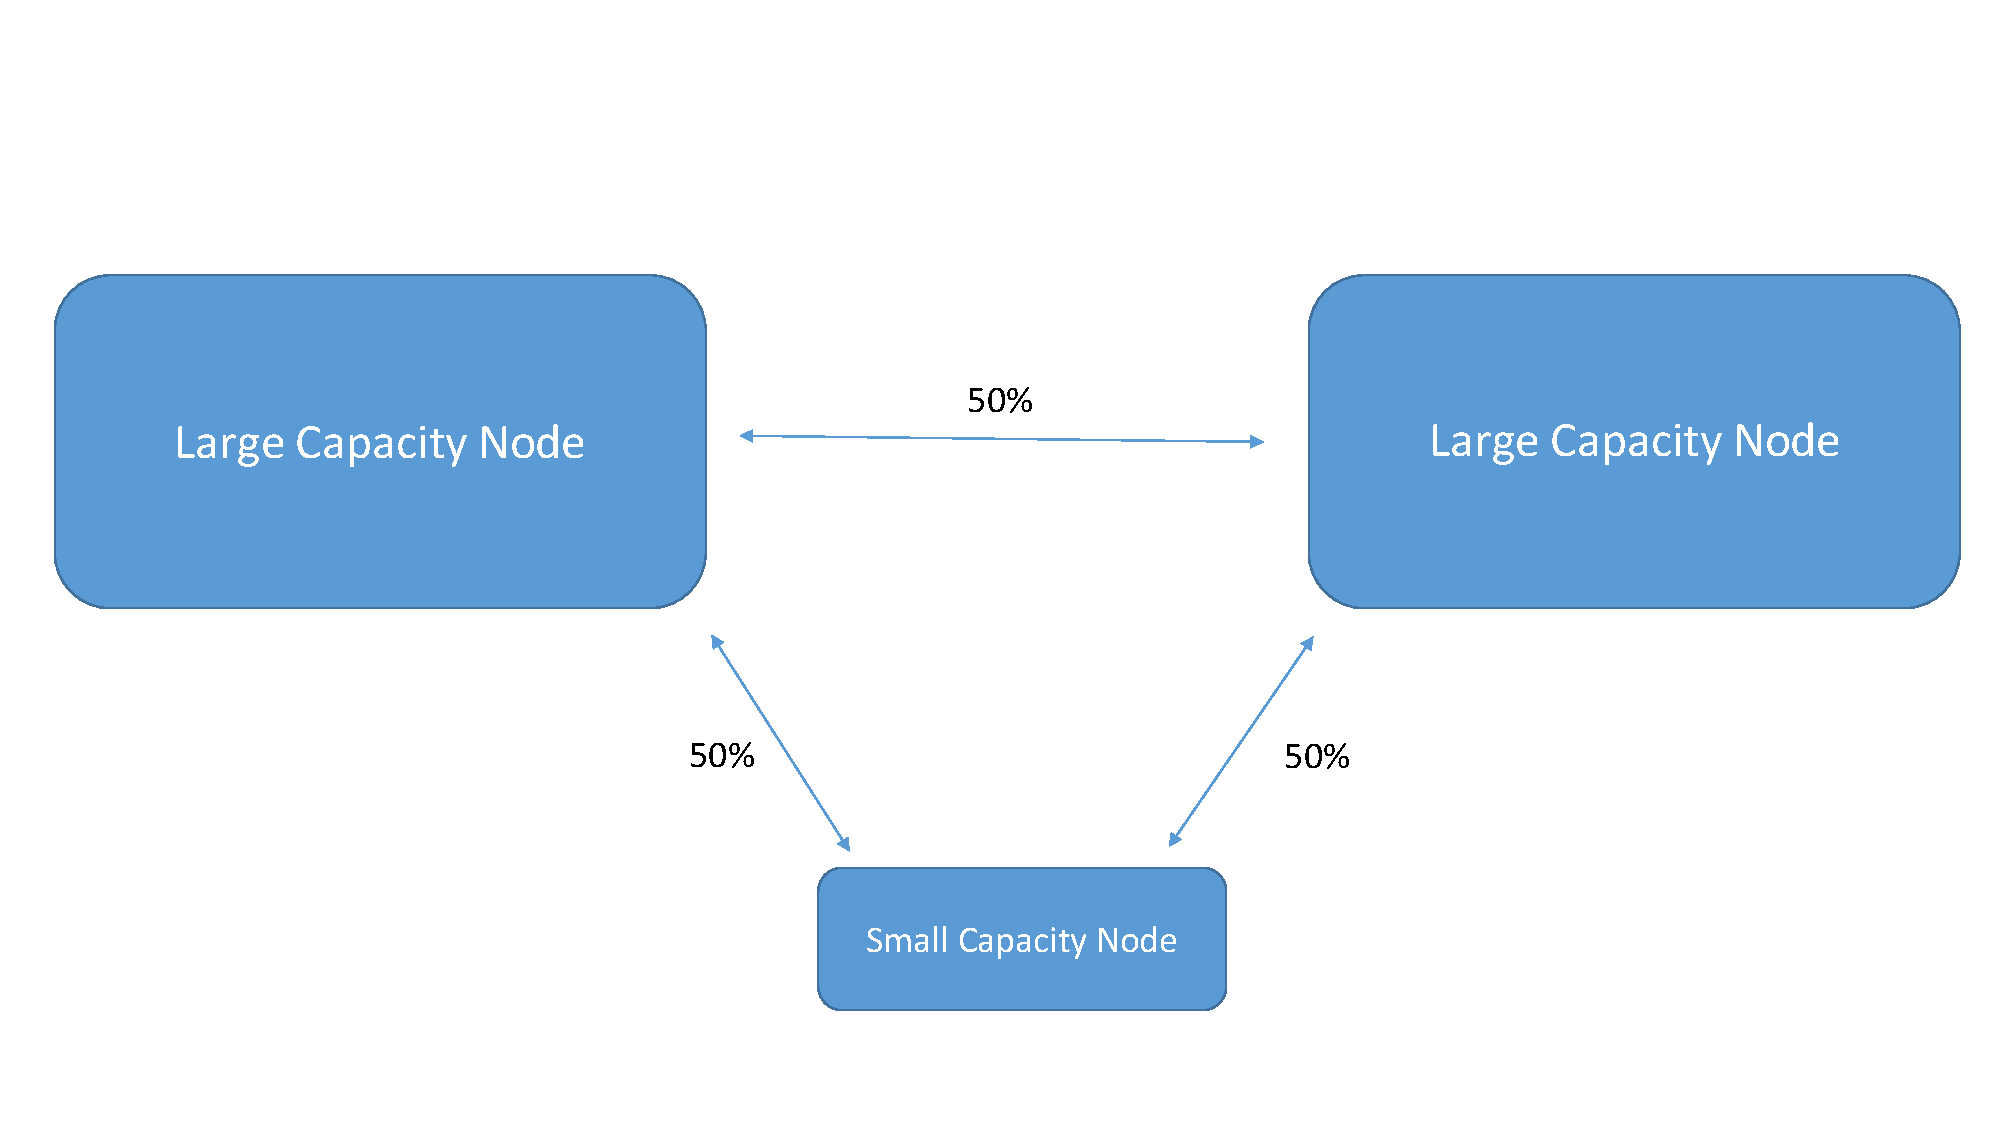
\includegraphics[scale=0.5]{images/homogeneous_tier_disparity.pdf} 
      \caption{A cluster with nodes of varying resource capacity.}
      \label{fig:tier_size_disparity}
    \end{figure}

  \subsection{Acropolis Base System}

  NDFS is facilitated by a clustering of controller virtual machines (CVMs)
  which reside, one per node, on each server in the cluster. The CVM presents
  via NFS (for VMWare's ESXi [14]), SMB (for Microsoft's Hyper-V [17]), or
  iSCSI (for Nutanix's AHV [1]) an interface to each hypervisor that they
  reside on. For example, the interface provided by the CVMs to VMware's ESXi
  hypervisor [14] will be interfaced with as a datastore. The virtual machines'
  virtual disk files will reside on the Nutanix datastore and be accessed via
  NFS through the CVM sharing a host with the user VM. Within the CVM exists an
  ecosystem of process that make up the ADSF. This work is scoped specifically
  to the I/O manager process, Stargate.


  \subsection{Stargate}

  The Stargate process is responsible for all data management and I/O
  operations. The NFS/SMB/iSCSI interface presented to the hypervisor is also
  presented by Stargate. All file allocations and data replica placement
  decisions are made by this process.

  As the Stargate process facilitates writes to physical disks, it gathers
  statistics for each disk such as the number of operations currently in flight
  on the disk (queue length), how much data in bytes currently resides on the
  disk, and average time to complete an operation on the disk. These statistics
  are only gathered on the local disks; however, they are then stored in a
  distributed database provided by another ADSF service along with the
  statistics gathered by every other Stargate in the cluster. These disk
  statistics stored in the database and are pulled periodically and are then
  used to make decisions on data placement when performing writes.

    \subsubsection{Oplog and Extent Store}

% TODO

    \subsubsection{Storage Tiering}

% TODO

    \subsubsection{Data Replication and Fault Tolerance}

% TODO

    \subsubsection{Replica Selection}

% TODO

%%%%%%%%%%%%%%%%%%%%%%%%%%%%%%%%%%%%%%%%%%%%%%%%%%%%%%%%%%%%%%%%%%%%%%%%%%%%%%%
\section{Prior Work}

% TODO

%%%%%%%%%%%%%%%%%%%%%%%%%%%%%%%%%%%%%%%%%%%%%%%%%%%%%%%%%%%%%%%%%%%%%%%%%%%%%%%
\section{Implementation}

% TODO

  \subsection{Overview}

% TODO

  \subsection{Fitness Values and Functions}

% TODO

  \subsection{Weighted Random Selection Algorithms}

% TODO

  \subsection{WeightedVector Class}

% TODO

  \subsection{Changes to the Stargate Disk Stats}

% TODO

  \subsection{Unit Testing}

% TODO

    \subsubsection{WeightedVector Unit Tests}

% TODO

    \subsubsection{ReplicaSelector Unit Tests}

%%%%%%%%%%%%%%%%%%%%%%%%%%%%%%%%%%%%%%%%%%%%%%%%%%%%%%%%%%%%%%%%%%%%%%%%%%%%%%%
\section{Results and Evaluation}

% TODO

  \subsection{Write Patterns and Fio}

% TODO

  \subsection{Experimental Setup}

% TODO

  \subsection{Low Outstanding Operation Test Results}

% TODO

  \subsection{High Outstanding Operation Test Results}

%%%%%%%%%%%%%%%%%%%%%%%%%%%%%%%%%%%%%%%%%%%%%%%%%%%%%%%%%%%%%%%%%%%%%%%%%%%%%%%
\section{User Guide}

% TODO

  \subsection{Re-creating Experiments}

% TODO

  \subsection{Scraping Data From the Nutanix Cluster}

%%%%%%%%%%%%%%%%%%%%%%%%%%%%%%%%%%%%%%%%%%%%%%%%%%%%%%%%%%%%%%%%%%%%%%%%%%%%%%%
\section{Conclusions}

% TODO

  \subsection{Summary}

% TODO

    \subsubsection{Low Outstanding Operation Test}

% TODO

    \subsubsection{High Outstanding Operation Test}

  \subsection{Conclusion}

    % Explain how this work solves the stated problems.

% TODO

  \subsection{Future Work}

% TODO

    \subsubsection{Real-time Fitness Feedback}

      % Realtime feedback from disks using historical latency numbers.
    
% TODO

    \subsubsection{Read Replica Selection}

      % Based on historical latencies.

% TODO

    \subsubsection{More Fitness Function Variables}

      % CPU, disk wear, data access patterns.

% TODO

%%%%%%%%%%%%%%%%%%%%%%%%%%%%%%%%%%%%%%%%%%%%%%%%%%%%%%%%%%%%%%%%%%%%%%%%%%%%%%%
\section{Appendix}

% TODO

  \subsection{Herding Behavior Due to Implementation Bug}

% TODO

  \subsection{Glossary}

% TODO

  \subsection{References}

% TODO


\end{document}
